\documentclass{beamer}[10]


%
% macro
%

\usepackage[orientation=landscape,size=custom,width=16,height=9,scale=0.5,debug]{beamerposter} 
\usepackage[beamer]{hf-tikz}
\usepackage{xfrac}
\usepackage[usenames,dvipsnames]{color}
\usepackage{makeidx}

%
% Macros
%

\definecolor{light-gray}{gray}{.80}
\definecolor{light-yellow}{rgb}{255,255,153}

% colorized font
\newcommand{\red}[1] { {\color{red} #1} }
\newcommand{\blue}[1] { {\color{blue} #1} }
\newcommand{\green}[1] { {\color{green} #1} }
\newcommand{\gray}[1] { {\color{gray} #1} }
\newcommand{\grey}[1] { {\color{gray} #1} }


% environments
\newminted{python}{mathescape} 
\newenvironment{theindex}
 {\let\item\par
  %definitions for subitem etc
  }{}
\newcommand\indexspace{}
\newenvironment{xframe}[2][]
  {\begin{frame}[fragile,environment=xframe,#1]
  \frametitle{#2}}
  {\end{frame}}
  
% python highlights: module, method
\newcommand{\pymodule}[1] { \textbf{#1} }
\newcommand{\pyfunction}[1] {\textit{#1}}
\newcommand{\keyword}[1] {\texttt{#1}}
\newcommand{\pyver}[1]{\colorbox{yellow}{#1}}
\newcommand{\pyvers}[1]{\raisebox{0em}{\colorbox{yellow}{#1}}}

% special symbils
\newcommand{\mymapsto}{\operatornamewithlimits{\longmapsto}}

\makeatletter
\newcommand{\xMapsto}[2][]{\ext@arrow 0599{\Mapstofill@}{#1}{#2}}
\def\Mapstofill@{\arrowfill@{\Mapstochar\Relbar}\Relbar\Rightarrow}
\makeatother

\newcommand{\code}[1] { \texttt{#1} }


%
% style
%

\setbeamercovered{transparent}
\mode<presentation>

%\geometry{top=5pt, margin=5pt}
%The outertheme defines the head and the footline of each slide
% \setbeamercolor{block title}{bg=orange}
% \useinnertheme{circles}
% \useoutertheme{split}
%\beamertemplatenavigationsymbolsempty

%\usetheme[numbers,totalnumber,compress,sidebarshades]{Babel}
\setbeamertemplate{headline}{
 \leavevmode%
  \hbox{%
%,bb=0 0 5cm 2cm
    \hskip5pt
    
\includegraphics[height=1.2cm]{babel-logo.eps}
    \hskip245pt
    
\includegraphics[height=1.2cm]{ep14-logo.eps}
    }
}
\setbeamertemplate{footline}{
    \centerline{
        \gray{
            Roberto Polli - \href{mailto:roberto.polli@babel.it}{roberto.polli@babel.it}
        }
    }
}
%\useinnertheme[shadow=false]{rounded}
% frametitle
\setbeamertemplate{frametitle}[default][center]
\setbeamercolor*{frametitle}{bg=white,fg=gray,parent=palette primary}
\setbeamerfont{frametitle}{series=\bfseries,size={\fontsize{16}{8}}}
%title
\setbeamercolor{title}{fg=black,bg=white}
\setbeamerfont{title}{series=\bfseries,size={\fontsize{24.88}{32}}}
%subtitle
\setbeamercolor{subtitle}{fg=gray}
\setbeamerfont{subtitle}{series=\bfseries,size={\fontsize{14}{}}}
%titlepage
\setbeamertemplate{title page}[default][center]
% bullets
\setbeamercolor{itemize item}{fg=gray}
\setbeamertemplate{itemize items}[circle]
\setbeamercolor{itemize item}{fg=light-gray}
\setbeamercolor{itemize items}{fg=light-gray}
% enumerations
\setbeamercolor{enumerate item}{fg=black}
\setbeamercolor{local structure}{fg=black}

%
% increase itemize spacing
%
%\newlength{\wideitemsep}
%\setlength{\wideitemsep}{\itemsep}
%\addtolength{\wideitemsep}{14pt}
%\let\olditem\item
%\renewcommand{\item}{\setlength{\itemsep}{\wideitemsep}\olditem}

  % \usecolortheme[named=orange]{structure}
  % \useinnertheme{circles}
  % \usefonttheme[onlymath]{serif}
  \setbeamercovered{transparent}
  % \setbeamertemplate{blocks}[rounded][shadow=true]

\makeindex


\title{Statistics 101 for System Administrators}
\subtitle{EuroPython 2014, $22^{th}$ July - Berlin}
\author{Roberto Polli - \href{mailto:roberto.polli@babel.it}{roberto.polli@babel.it}}
\date{22 July 2014}
\institute{Babel Srl P.zza S. Benedetto da Norcia, 33\\ 
    00040, Pomezia (RM) - www.babel.it}

%
%
\begin{document}

%% cover
\frame{\titlepage 
\vspace{-0.5cm}
}

%% agenda
\iffalse
\frame{\frametitle{Agenda}
\tiny
\tableofcontents%[pausesection]
}
\fi

%\section{Test}
\usepackage{pdfcomment}

\begin{pyframe}{Title}
Antani
module: \pymodule{subprocess, psutil}
symbols: $\clubsuit \diamondsuit \heartsuit \spadesuit$
\end{pyframe}

\begin{pyframe}{\pyoptional{Test Slide with styles}}
\begin{itemize}
\item Bullet \index{Bullet} item 0 $a_i + b_j = 10 $
\item Bullet \index{Bullet} item 2 with code\footnote{Do you like footnotes?}
\begin{pycode*}{escapeinside=||}
    # footnotesize
    for  a in range(10):
        yield a
    # $\xmapsto[encode]{utf-8}$
    # $a \rightarrow b^{c}$
    |\index{return}return| False
\end{pycode*}
\item Bullet Item 3 
\end{itemize}
\end{pyframe}

\begin{pyframe}{Test Slide with styles}
\begin{enumerate}
\item Enumerate1 \index{enumerate} \pdfcomment{Pdf Comment Test Slide with styles}
    \begin{enumerate}
    \item EnumerateA  \pyver{w\"urstel re}sults
    \item \texttt{Inline minted ipython}
    \item Una linea 
    \item w\"urstelstra\ss e
    \end{enumerate}

\item Enumerate2 \`{e} 
 [\red{196}, \blue{168}] 
\begin{pycode*}{escapeinside=||}
@|\pyver{decorator}|
def foo(tmp):
    def bar(*args):
        |\index{return}return| tmp(|$*args_{i}$|)
    |\index{return}return| bar
\end{pycode*}

\end{enumerate}

\end{pyframe}

\begin{pyframe}{Tabular and image}
A Tabular follows \\
\begin{tabular}{|c|c|}\hline
Cell 1 & Cell 2 \\
\hline 
\end{tabular}
\\
\begin{table}
\begin{tabular}{|c|c|}\hline
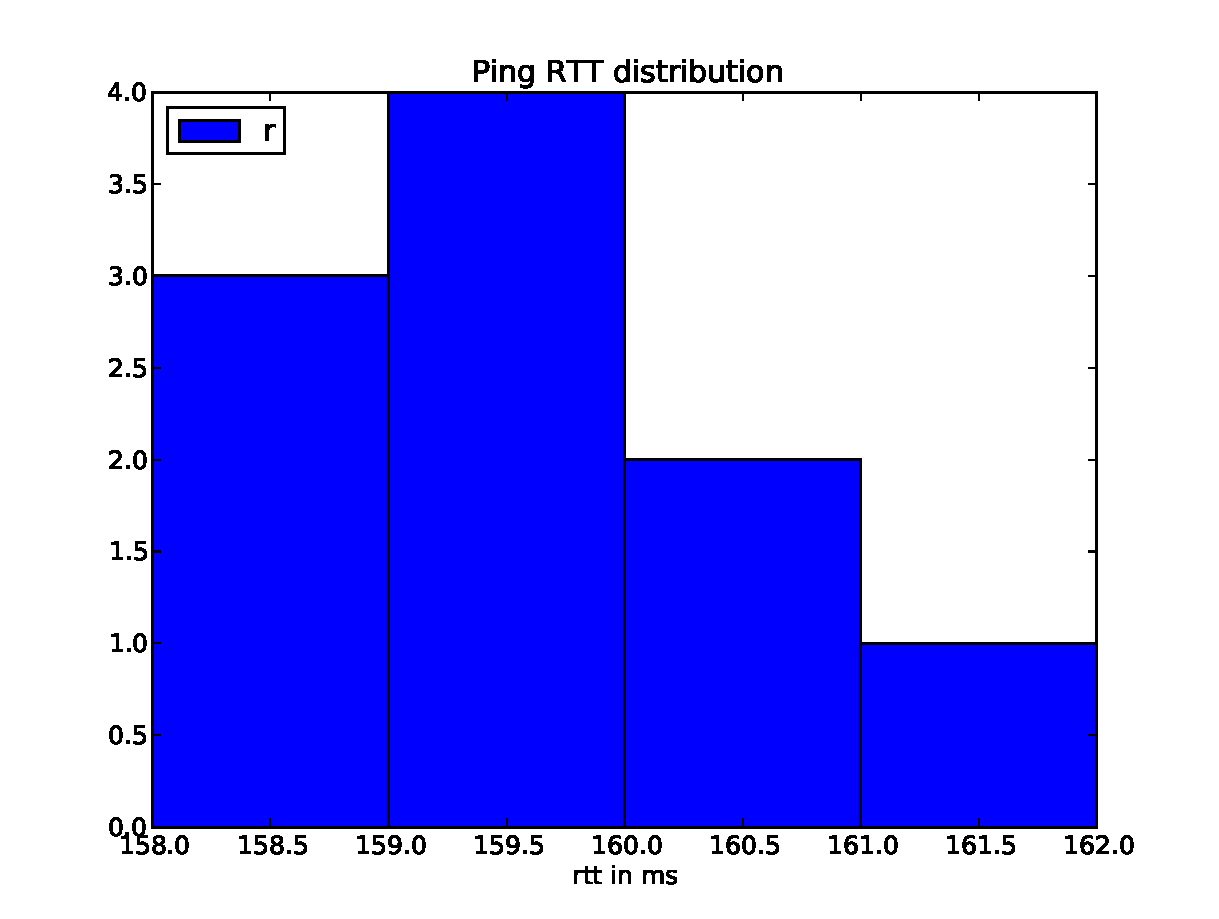
\includegraphics[height=4cm]{ping_distribution.pdf}   & 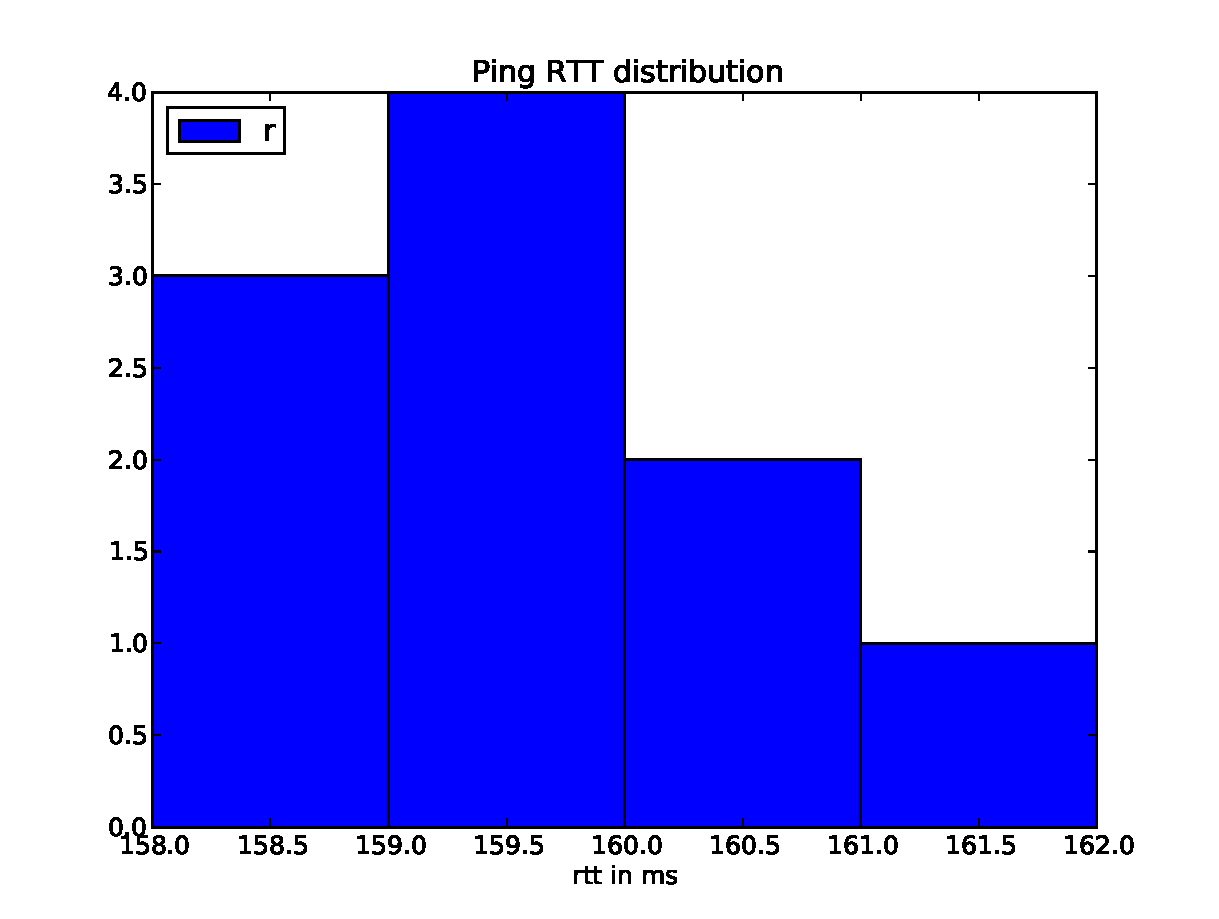
\includegraphics[height=4cm]{ping_distribution.pdf}  \\
\hline 
\end{tabular}
\end{table}
\end{pyframe}

\begin{pyframe}{Simple Column}
\begin{columns}
\column[t]{6cm}
\begin{pycode}
"""using set and dict
"""
distro = {x: rtt.count(x) 
  for x in set(rtt)}
# or using a
from collections import defaultdict
distro = defaultdict(int)
for x in rtt:
    distro[x] += 1
    

\end{pycode}
\column[t]{5cm}
-skip-\\
-skip-\\
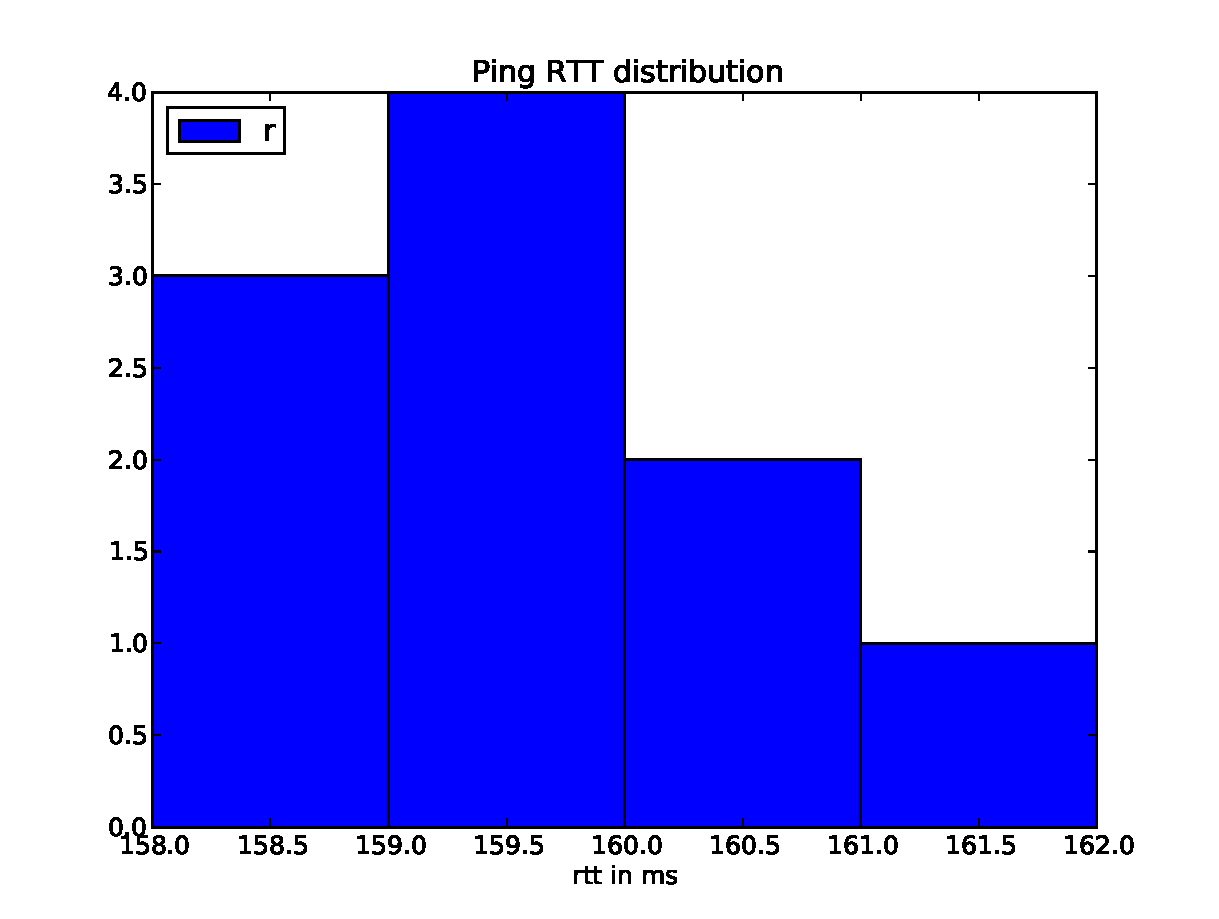
\includegraphics[height=4cm, width=4dm]{ping_distribution.pdf}  
\end{columns}
\end{pyframe}


\begin{pyframe}{2-columns and verbatim}
Two columns
\begin{columns}

\column[t]{5cm}
1
2
3
\begin{verbatim}
4
5
6
\end{verbatim}

\column[t]{5cm}
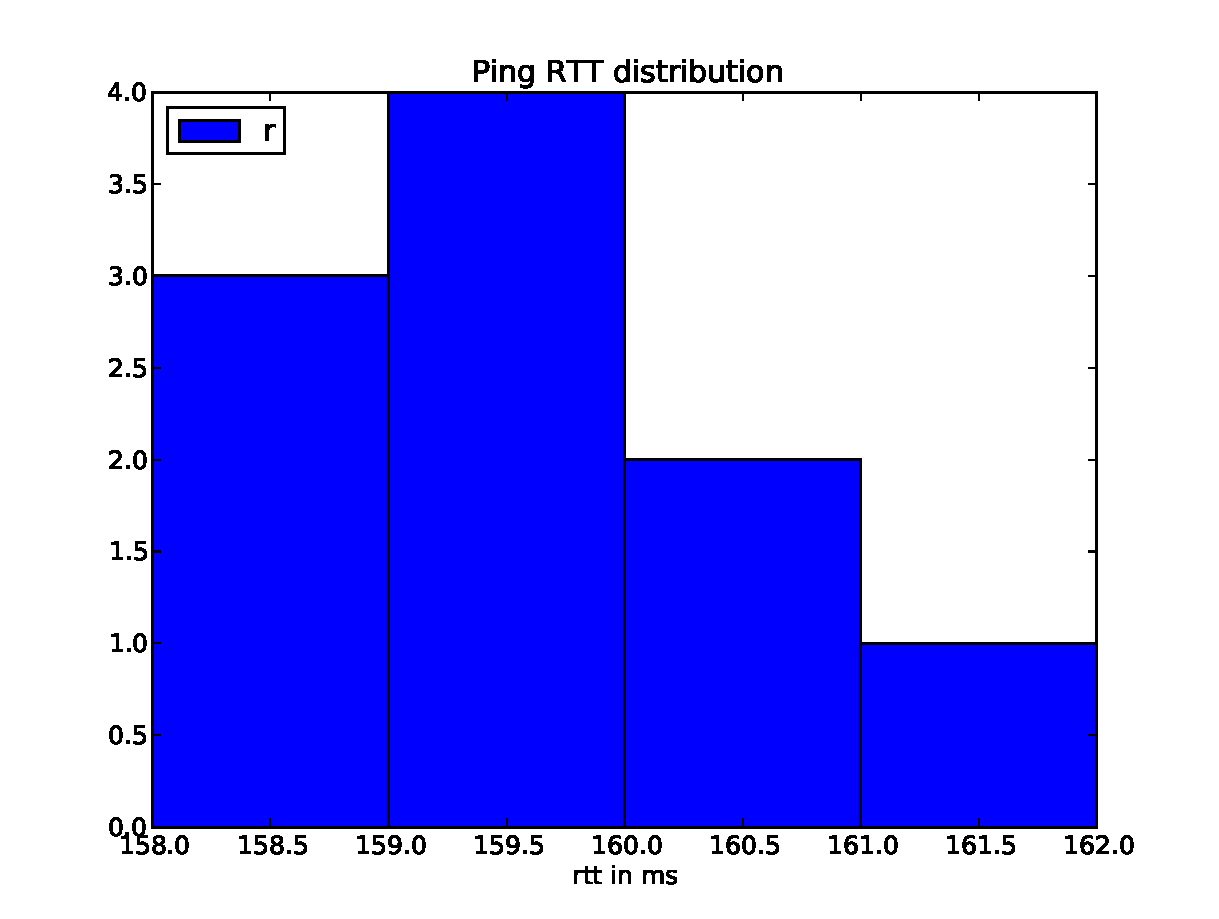
\includegraphics[height=4cm,width=5cm]{ping_distribution.pdf}  
\end{columns}

\end{pyframe}



\begin{pyframe}{Simple processing: distribution}
\begin{columns}
\column[t]{6cm}
\begin{pycode}
"""using set and dict """
distro = {x: rtt.count(x) 
  for x in set(rtt)}
# or using a
from collections import defaultdict
distro = defaultdict(int)
for x in rtt:
    distro[x] += 1
\end{pycode}
\column[t]{4cm}
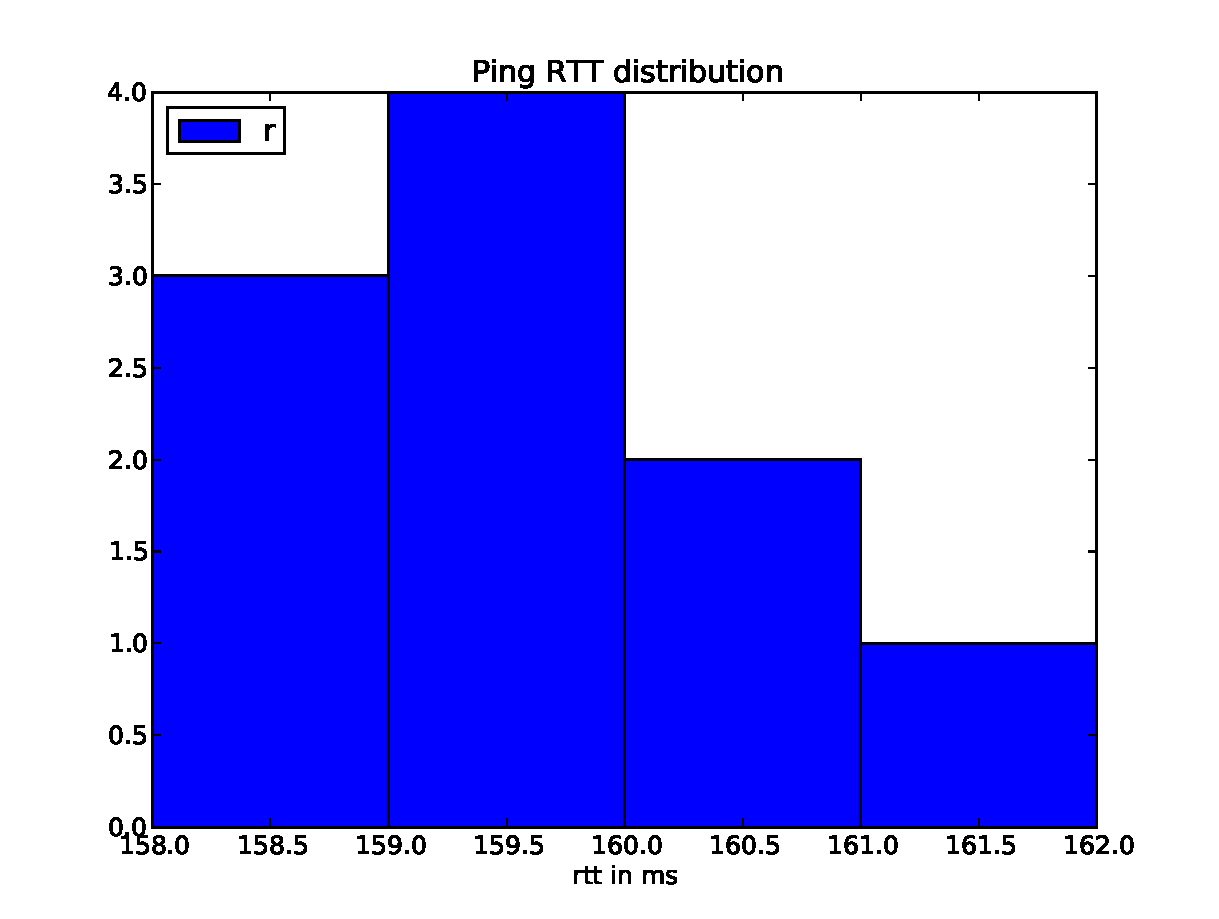
\includegraphics[width=4cm,height=4cm]{ping_distribution.pdf}  
\end{columns}
\end{pyframe}

\begin{pyframe}{Index}

fooo bar

\end{pyframe}


\section{Intro}
\frame{ \frametitle{Who? What? Why?}
\begin{itemize}

\item Using (and learning) elements of statistics with python.

\item Roberto Polli - Community Manager @ Babel.it. Loves writing in C,
Java and Python. Red Hat Certified Engineer and Virtualization
Administrator.

\item Babel – Proud sponsor of this talk ;) Delivers large mail
 infrastructures based on Open Source software for Italian ISP and
 PA\@. Contributes to various FLOSS.
\end{itemize}
}

\begin{pyframe}{Agenda}
\begin{itemize}
\item A latency issue: what happened?
\item Correlation in 30" 
\item Combining data
\item Plotting time
\item modules: \pymodule{scipy, matplotlib}
\end{itemize}
\end{pyframe}


\begin{pyframe}{A Latency Issue}
\begin{itemize}
\item Episodic network latency issues
\item Logs traces: message size, \#peers, retransimissions
\item Do we need to scale? Was a peak problem? 
\end{itemize}
Find a rapid answer with python!
\end{pyframe}

\iffalse
\begin{pyframe}{Gathering data}
The most time-consuming part of the analysis
\begin{itemize}
\item Parse log file with a strategy
\item Collect log samples and tinker in ipython
\item Write simple parsing library with tests
\end{itemize}
Curious? Attend `Python for System Administrators' on 24 July
\end{pyframe}
\fi
\iffalse
\begin{pyframe}{Gathering data}
\begin{pycode}
# Use dict + zip to convert
data = [('timestamp', 'late', 'retry', 'size', 'peers'),
(1379703191, 0.12, 2, 1, 123, 2313),
(1379703192, 12.43, 0, 1, 3223, 2303),
...
(1379 709000, 0.43, 0, 1, 3223, 2303)
]
# in
table = dict(zip(data[0],  zip(*data[1:]) ))
> { 'timestamp' : [ 1379703191, 1379703191, ..., 1379709000],
'late': [0.12, 12.43, ..., 0.43],
... }

\end{pycode}
\end{pyframe}
\fi


\begin{pyframe}{Basic statistics}
Python provides basic statistics, like
\begin{pycode}
from scipy.stats import mean	# $\bar{x}$
from scipy.stats import std	# $\sigma_{X}$
T = { 'ts': (1, 2, 3, .., ),
      'late': (0.12, 6.31, 0.43, .. ),
      'peers': (2313, 2313, 2312, ..),...}
      
print([k, max(X), min(X), mean(X), std(X) ]   
        for k, X in T.items() ])
\end{pycode}
\end{pyframe}



\begin{pyframe}{Distributions}
Data distribution - aka $\delta_{X}$ - shows event frequency.
\begin{columns}
\column[t]{.6\textwidth} 
\begin{pycode}
# The fastest way to get a 
#  distribution is
from matplotlib import pyplot as plt
freq, bins, _ = plt.hist(T['late'])

# plt.hist returns a
distribution = zip(bins, freq)
\end{pycode}
\column[t]{.4\textwidth} 
A ping rtt distribution
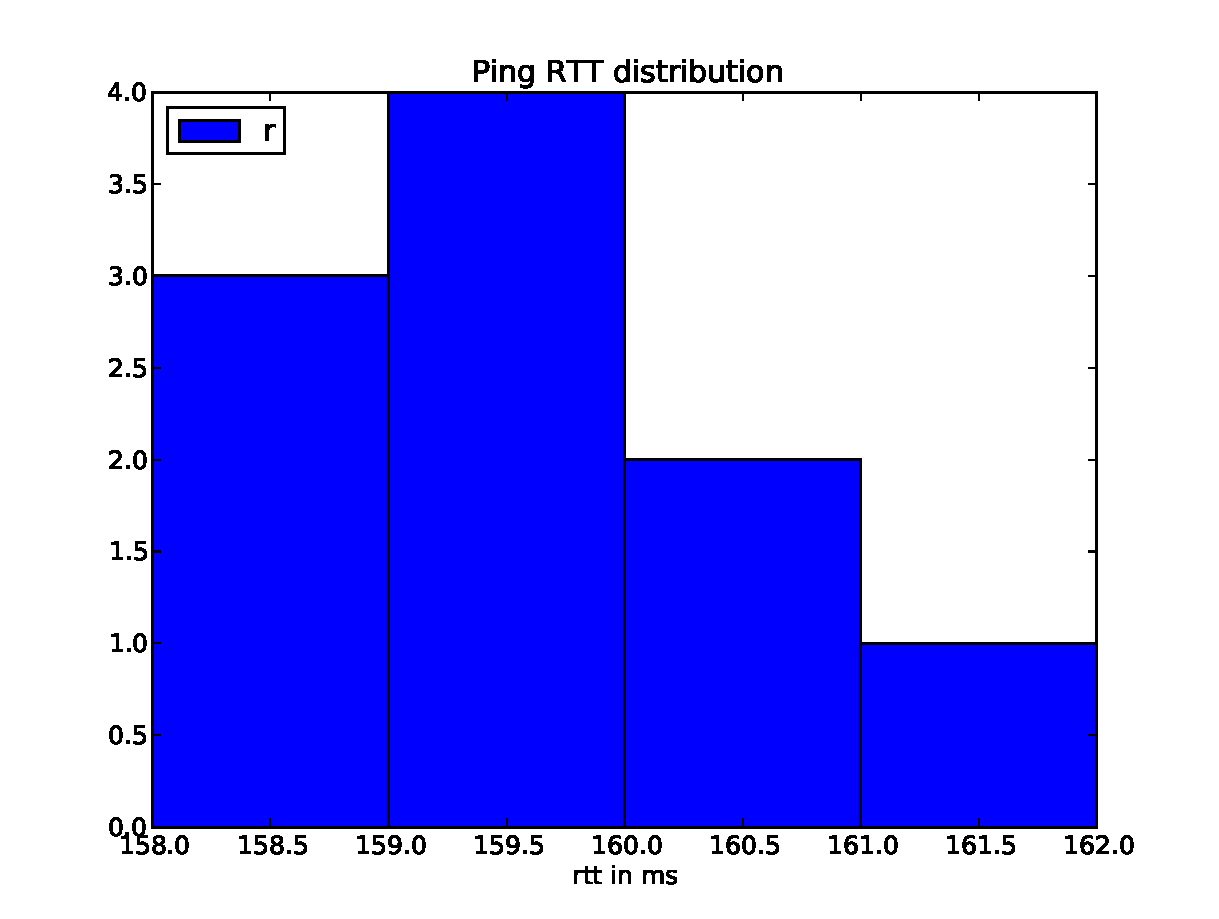
\includegraphics[width=6cm]{ping_distribution.pdf}
\end{columns}
\end{pyframe}

\iffalse
\begin{pyframe}{Time and Size distribution}
Frequency can be calculate on time or size
Time distribution: mail sent in 4hours bucket
\begin{pycode}
from matplotlib import pyplot as plt
frequency, values, _  = plt.hist(T['late'])
zip(values, frequency)
\end{pycode}
\includegraphics[width=5cm,height=5cm]{distribution.pdf}
\end{pyframe}
\fi

\begin{pyframe}{Correlation I}
Are two data series $X, Y$ related? \\
Given 
\begin{formula}
\Delta x_{i} = x_{i} - \bar{x}
\end{formula}
Mr. Pearson answered with this formula
\begin{equation}
\rho(X, Y) = \frac{ \sum_{i} \Delta x_{i} \Delta y_{i} }{ \sqrt{ \sum_i \Delta^{2} x_i \Delta^{2} y_i } } \in [-1, +1]
\end{equation}
$\rho$ identifies if the values of $X$ and $Y$ `move' together \emph{on the same line}.
\end{pyframe}

\begin{pyframe}{You must (scatter) plot}
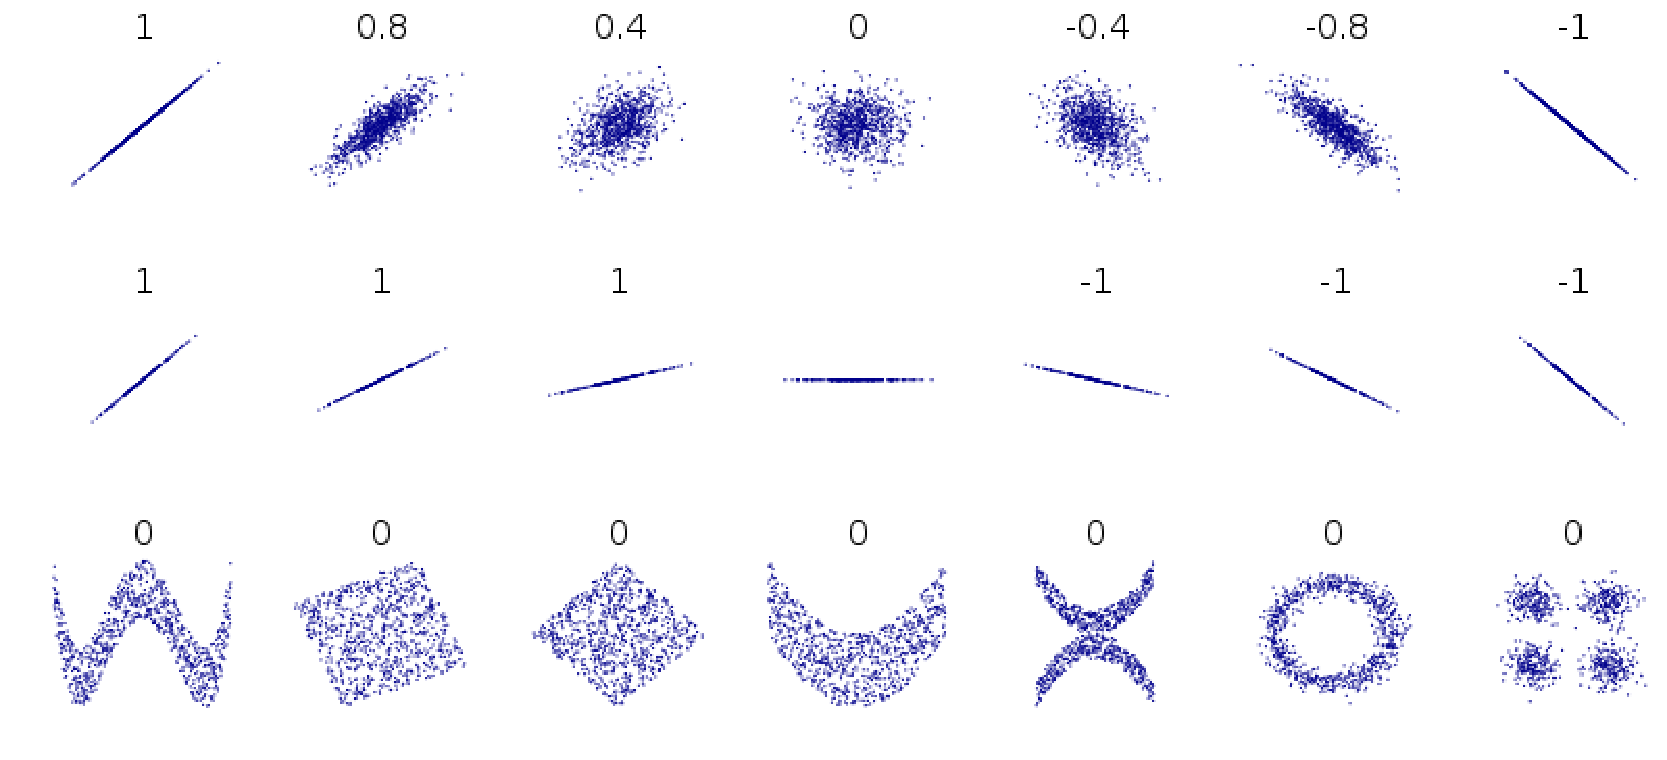
\includegraphics[height=5.5cm]{correlation.pdf}
{\large
\begin{center}
$\rho$ doesn't find non-linear correlation!
\end{center}
}
\end{pyframe}


\begin{pyframe}{Probability Indicator}
Python \pymodule{scipy} provides a correlation function,
returning two values:
\begin{itemize}
\item the $\rho$ correlation coefficient   $\in [-1, +1]$
\item the $probability$ that such datasets are produced by uncorrelated systems
\end{itemize}
\begin{pycode}
from scipy.stats.stats import pearsonr # our beloved $\rho$
a, b = range(0, 100), range(0, 400, 4)
c, d = [randint(0, 100) for x in a], [randint(0, 100) for x in a]
correlation, probability = pearsonr(a,b) #  $\rho=1.000, p=0.000$
correlation, probability = pearsonr(c,d) # $\rho=-0.041, p=0.683$
\end{pycode}
\end{pyframe}

\begin{pyframe}{Combinations}
\pymodule{itertools} is a gold pot of useful tools.

\begin{columns}
\column[t]{.7\textwidth}
\begin{pycode}
from itertools import combinations
# returns all possible combination of
#  items grouped by N at a time
items = "heart spades clubs diamonds".split()
combinations(items, 2)

# And now all possible combinations between
#  dataset fields!
combinations(T, 2)
\end{pycode}
\column[t]{.3\textwidth}
Combinating 4 suites, 2 at a time.\\
\begin{center}
\\
\hearts \spades \\
\hearts \clubs \\
\hearts \diamonds \\
\spades \clubs \\
\spades \diamonds \\
\clubs \diamonds \\
\end{center}
\end{columns}
\end{pyframe}



\begin{pyframe}{Netfishing correlation I}
\begin{pycode}
# Now we have all the ingredients for
#  net-fishing relations between our data!
for (k1,v1), (k2,v2) in combinations(T.items(), 2):
  # Look for correlations between every dataset!
  corr, prob = pearsonr(v1, v2)
  
  if corr > .6:
    print("Series", k1, k2, "can be correlated", corr)
  elif prob < 0.05:
    print("Series", k1, k2, "probability lower than 5%%", prob)
   
\end{pycode}
\end{pyframe}


\begin{pyframe}{Netfishing correlation II}
Now plot all combinations: there's more to meet with eyes!
\begin{pycode}
# Plot everything, and insert data in plots!
for (k1,v1), (k2,v2) in combinations(T.items(), 2):
    corr, prob = pearsonr(v1, v2)
    plt.scatter(v1, v2)

    # 3 digit precision on title
    plt.title("R={:0.3f} P={:0.3f}".format(corr, prob))
    plt.xlabel(k1); plt.ylabel(k2)

    # save and close the plot
    plt.savefig("{}_{}.png".format(k1, k2)); plt.close()   
\end{pycode}
\end{pyframe}

\begin{pyframe}{Plotting Correlation}
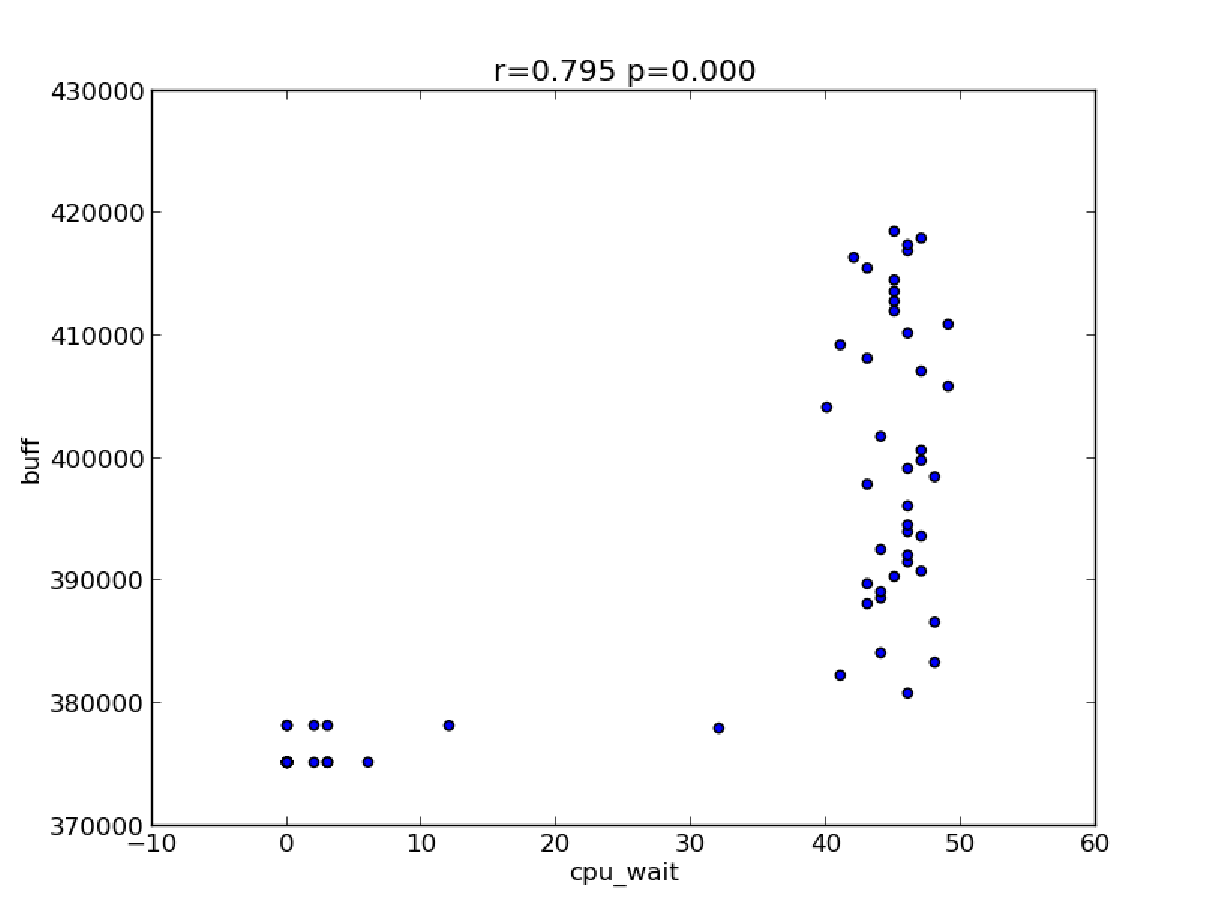
\includegraphics[height=6.6cm,width=12cm]{monochromo_cpu_wait_buff.pdf}
\end{pyframe}

\begin{pyframe}{Color is the 3rd dimension}
\begin{pycode*}{escapeinside=||}

from itertools import cycle
colors = cycle("rgb")   # use more than 3 colors!
labels = cycle("morning afternoon night".split())
size = datalen / 3      # 3 colors, right?
for (k1,v1), (k2,v2) in combinations(T.items(), 2):  
  [    plt.scatter(|\pyver{t1[i:i+size]}|, t2[i:i+size], 
        color=next(colors), 
        label=next(labels)
        ) for i in range(0, datalen, size) ]
  # set title, save plot & co

   
\end{pycode*}
\end{pyframe}

\iffalse
\begin{pyframe}{Example Correlation}
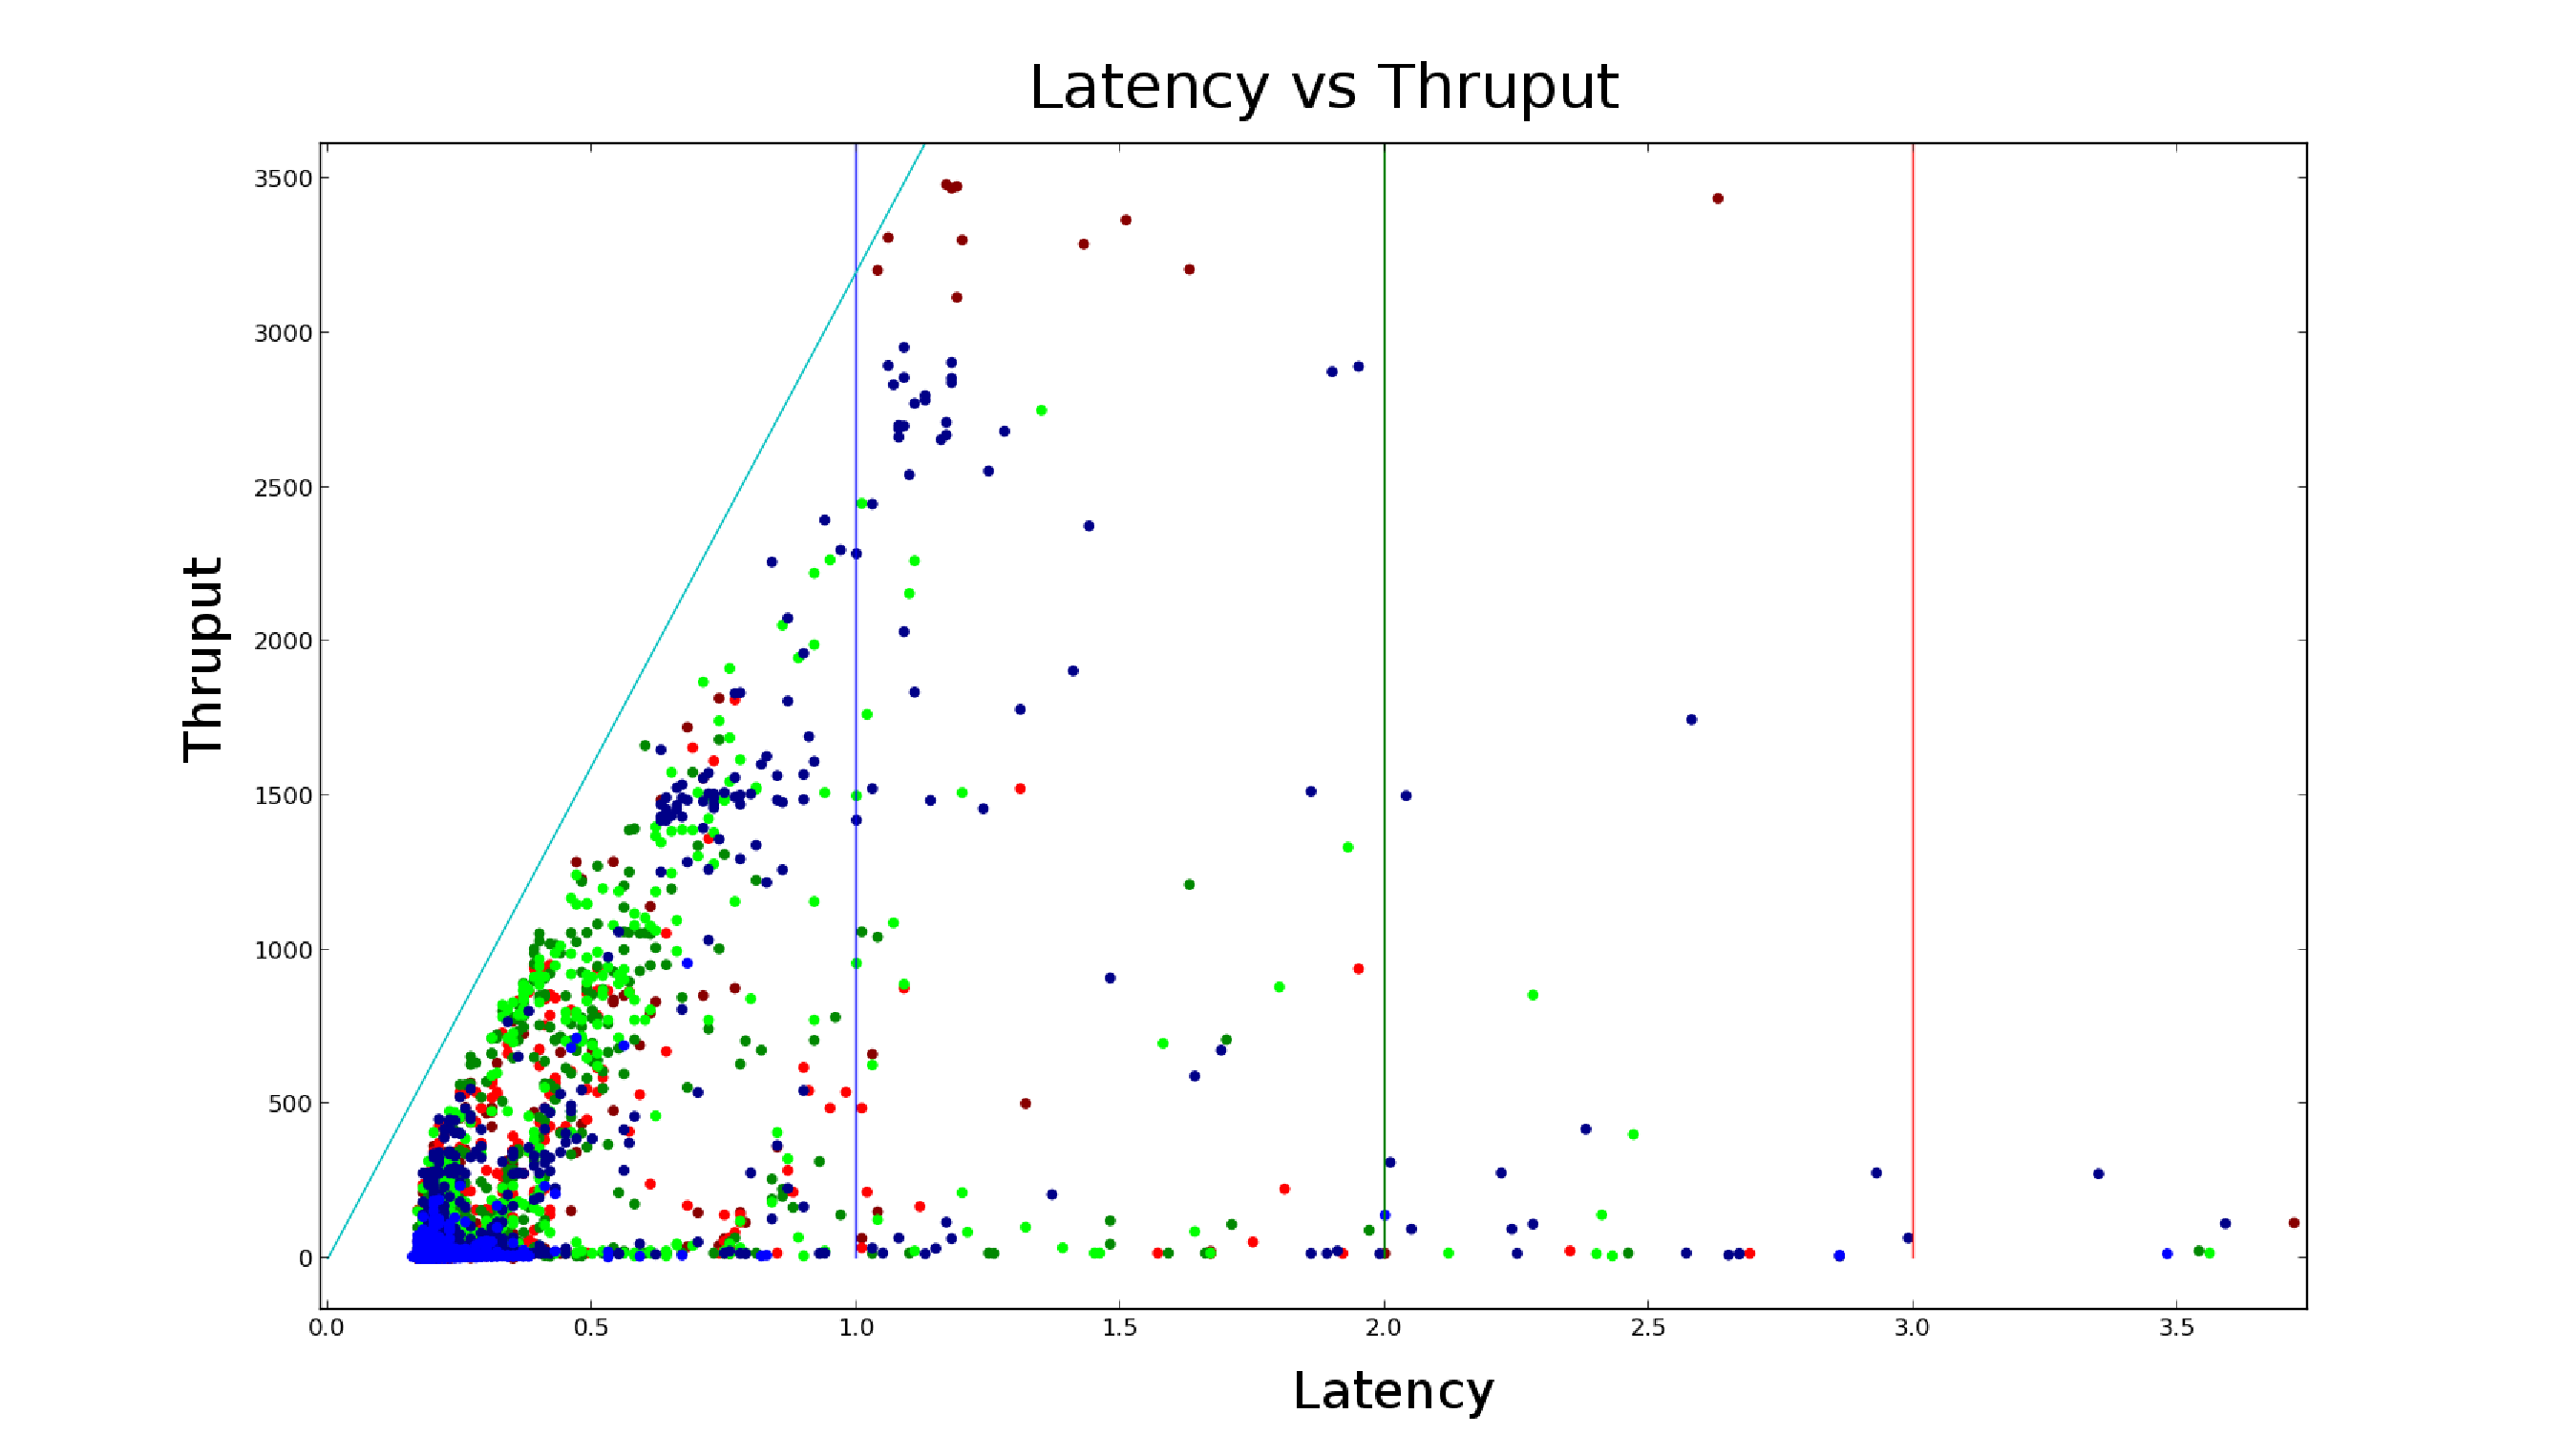
\includegraphics[height=7cm,width=15cm]{latency_thruput_colored.pdf}
\end{pyframe}
\fi

\begin{pyframe}{Example Correlation}
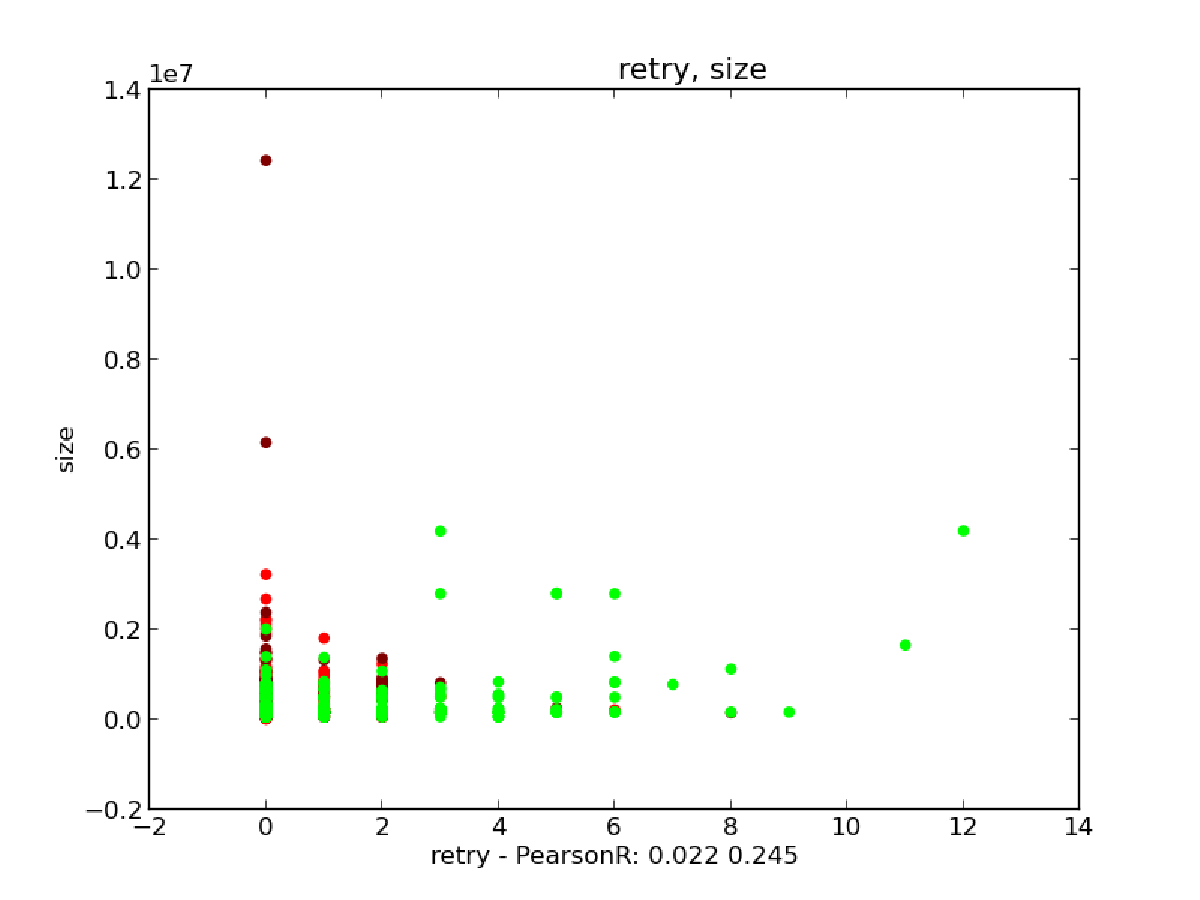
\includegraphics[height=7cm,width=15cm]{retry_size_colored.pdf}
\end{pyframe}


\begin{pyframe}{Latency Solution}
\begin{itemize}
\item Latency wasn't related to packet size or system throughput
\item Errors were not related to packet size
\item Discovered system throughput 
\end{itemize}
\end{pyframe}


\begin{pyframe}{Wrap Up}
\begin{itemize}
\item Use statistics: it's easy
\item Don't use $\rho$ to \emph{exclude} relations
\item Plot, Plot, Plot
\item Continue collecting results
\end{itemize}
\end{pyframe}

\begin{pyframe}{That's all folks!}
\begin{center}
Thank you for the attention! \\\\
\insertauthor
\end{center}
\end{pyframe}


\end{document}
